\documentclass[12pt]{article}
\usepackage{fullpage,enumitem,amsmath,amssymb,graphicx}

\begin{document}

\begin{center}
{\Large AI Agent for Lunar Lander}

\begin{tabular}{rl}
Prabhjot Singh Rai [prabhjot], Abhishek Bharani [abharani], Amey Naik [ameynaik]
\end{tabular}
\end{center}

\section{Task Definition}

\subsection{Scope}

The task accomplished by this project is to build an AI agent which would land with constant high rewards on a landing pad, defined by Box2D Lunar Lander available on OpenAI gym. This is accomplished by Reinforcement Learning, particularly by applying different Q-learning techniques. This project has explored Full DQN, Double DQN and Dueling Network Architecture (Dueling DQN), their performances in "solving" the game. 

\subsection{Evaluation}

We have considered a game to be solved when the agent starts getting average reward of 200 over 100 consecutive episodes. Performances have been compared with baselines and oracle. Moreover, we have also tried to get comparable results with the leader-board on OpenAI gym.

\section{Infrastructure}

We have used OpenAI library as our infrastructure. Although some insights are provided in Box2D Lunar Lander on OpenAI website, but thorough exploration of actions, state space, environment etc. were done before starting to solve the problem. Following is the description:

\subsection{Actions}
In this game, four discrete actions are available to the playing agent at any time frame: 

\begin{enumerate}[label=(\alph*)]
\item Do nothing
\item Fire left orientation engine (rotates the lunar lander clockwise)
\item Fire main engine (provides upward thrust)
\item Fire right orientation engine (rotates the lunar lander anti-clockwise)
\end{enumerate}

The agent can choose only one action among the given actions at a given time frame.

\subsection{Terrain} 
The terrain is a combination of 10 points, and the helipad(landing zone) is fixed between 5th and 6th points towards the center. The values of the height of the landing zone(5th and 6th points on the terrain) are viewport height divided by 4, and the rest of the points are randomly sampled between 0 to H/2 using \textit{numpy} random and smoothened (averaging 3 continuous points).

\subsection{Initial State}

The state is 8 dimensional values of different parameters of the lunar lander at any given time. The starting state is randomly initialized (the lunar lander takes a step in the world through the "idle" action) with certain bounds based on the environment.

Inspecting code of open\_ai lunar lander, we see that the initial states are defined by simulating the environment in one frame (calling box world simulation using time step as $1/FPS$). Using this simulation, elaborating the initial state as follows:

\begin{enumerate}
\item Position X (Initial Position X: final x which changed from half of viewport width to a value after taking "idle" action before the simulation)
\item Position Y (Initial Position Y: final y which changed from from the viewport height to a value after taking "idle" action before simulation)
\item Velocity X (Initial Velocity X: final velocity x changed from 0 to a value after taking "idle" action before simulation)
\item Velocity Y (Initial Velocity Y: final velocity y which changed from 0 to a value after taking "idle" action before simulation)
\item Current lander angle (Initial lander angle: final lander angle after simulation on "idle" action from 0 degrees)
\item Angular velocity (Initial angular velocity: final angular velocity after simulation on "idle" action from 0 angular velocity)
\item Left leg contacted the surface (Initial value: False, since there's is no probability that the lunar lander's leg will touch the moon surface when at the top)
\item Right leg contacted the surface (Initial value: False)
\end{enumerate}

\subsection{End State}

The episode ends in the following scenarios:

\begin{enumerate}
\item  When the lunar lander goes outside of the viewport bounds, the game is over with -100 is negative reward.
\item  When the lunar lander touches the ground with a high velocity
\item When the lunar lander touches the ground with body part except the legs
\item When the lunar lander stabilises on the moon's surface (change in shape of lunar lander is constantly 0 for a number of frames)
\end{enumerate}

\subsection{Rewards and Transitions}

Before defining the rewards, let's define the shape of the lunar lander which decides the rewards. The shape of the lunar lander is a function of position coordinates $(x, y)$, linear velocities $(v_x, v_y)$, lander angle $\theta$ and contact of both the lander legs. We are interested in finding the change of shape at every step for the lunar lander to calculate the rewards for each given action. Shape change is given by subtraction of previous shape and current shape. Formally, shaping at time frame $t$:

\begin{align*}
\text{shaping}_{t} = &- 100*(x^2 + y^2) \\
           & - 100*(v_x^2 + v_y^2) \\
            &- 100*abs(\theta) + 10*(\text{Left leg contacted}) + 10*(\text{Right leg contacted}) \\
\text{shape change} = & \text{shaping}_t - \text{shaping}_{t-1}
\end{align*}

The rewards are defined as follows:

\begin{enumerate}
\item If the lunar lander crashes, or goes out of the bounds: $-100$
\item If the lunar lander is not awake anymore (stabilises at 0 shape change): $+100$
\item Doing nothing: shape change 
\item Firing the engine: shape change - 0.3
\item Rotating: shape change - 0.03
\end{enumerate}

The total reward will automatically be a sum of all the rewards at each time frame, and if the lander touches the ground with it's legs, will add those rewards to the total rewards earned during an episode. Transition probabilities are unknown, we get next states by simulating the lunar lander in the box environment given the current state and action taken. \\

\textbf{Note}: The transition probabilities and rewards are unknown to our agent, which it will try to figure out through exploration and incorporate in learning. 


\section{Approach}

\subsection{Challenges}

We dedicated time to understand how the openai-gym is working internally. For this specific problem, we understood how the rewards and environment is behaving on every episode, as described in infrastructure. Moreover, to get faster results, we focused on better machine and GPU settings on google cloud and getting docker environment setup for codalab and reproducibility across platforms.

\subsection{Modelling the problem}

Basic framework is defined in Fig 1. The agent performs action($a$) on the environment. Performing the action on the environment returns reward($r$) and new state $s'$. Our agent then incorporates this information.

\begin{figure}%
\centering
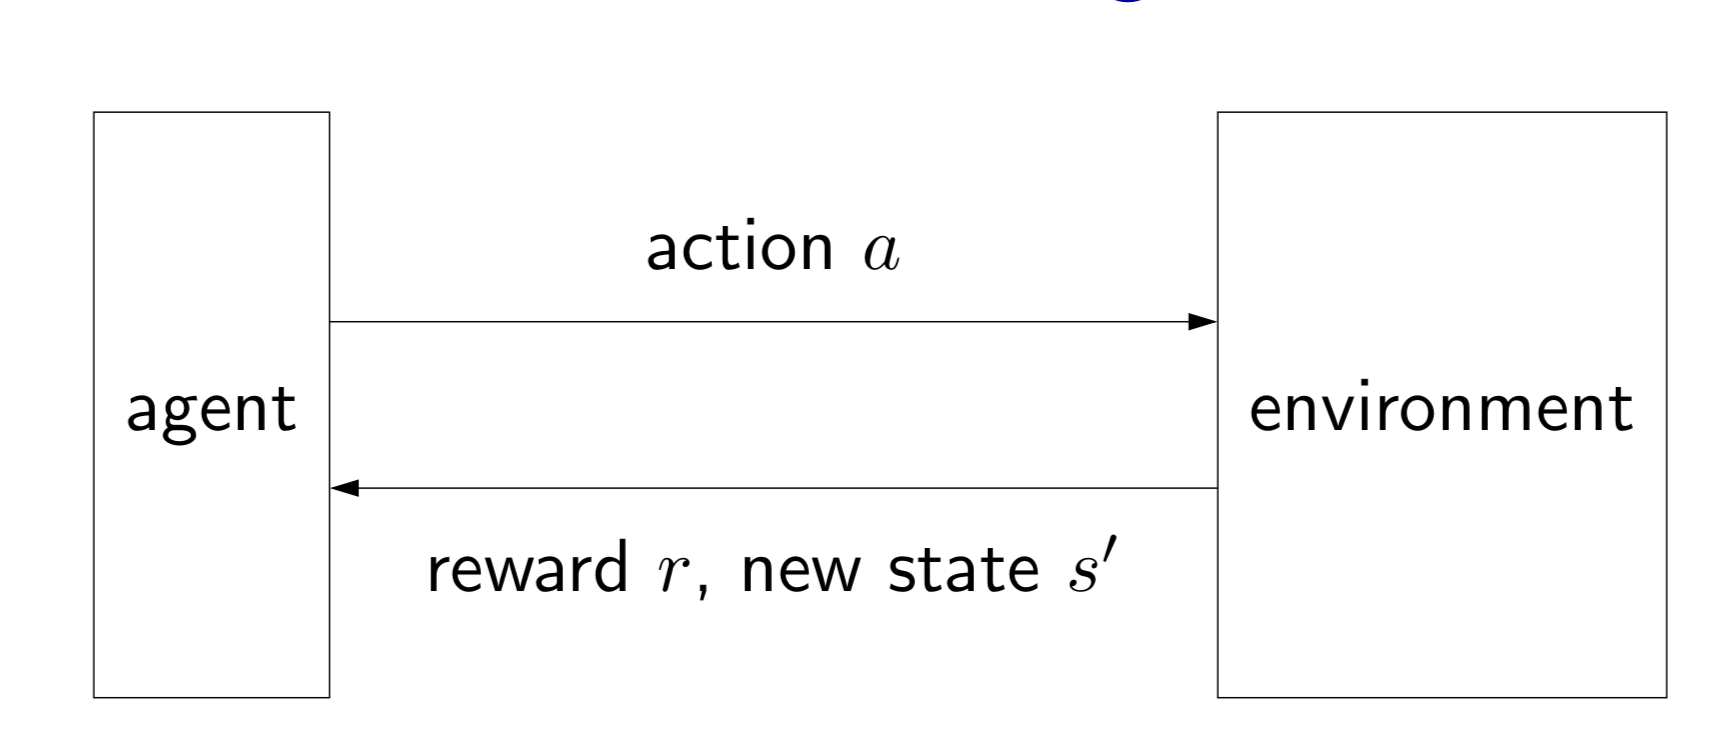
\includegraphics[scale=0.3]{reinforcement_framework.png}%
\caption{Reinforcement Learning framework}%
\label{fig:datastats}%
\end{figure}

In such a model, for our problem, here is quick description of notations:
\begin{enumerate}
\item $S$ is defined as all possible states, $s$ is one particular 8 dimensional state
\item $A$ is defined as all possible actions, $a$ is one of the actions out of $[\text{idle}, \text{fire engine}, \text{rotate left}, \text{rotate right}]$
\item $R$ is the reward distribution given $(s, a)$
\item $P$ is the set of possible transitions and their probabilities given $(s, a)$
\item $\gamma$: the discount factor. How much we want our agent to discount future reward. It is a hyperparameter that we define ourselves.
\end{enumerate}

Our model builds off of Q-learning algorithms by using a Deep Neural Network (DNN) for approximating the state-action Q-value, Q(s, a). 
Given the state $s$, our goal is to identify a policy $\pi_{opt}$ that maps the states to actions in order to maximize the total reward we get.

\begin{center}
S $\rightarrow$ A based on $\pi_{opt}$
\end{center}

As we know, $Q$ value is defined as the expected reward that we get following action $a$ in a given state $s$ and then following the policy $\pi$, our objective is to define a $Q_{opt} (s, a)$, which can be maximised over all possible actions at a state $s$, in order to find the $\pi_{opt}$.

\subsection{Approaches and Equations}

// Describe all equations (Amey)

\subsection{Accuracy and Efficiency Trade-off}

For our solutions, accuracy can be considered as consistency in getting more than 200 scores over a period of episodes. And efficiency would be how sooner we can get such weights for which the agent scores more than 200 scores. \\

When we train for more number of episodes (low efficiency), we get high accuracy (drop between consecutive episodes is lesser). And vice versa, if we stop early, we are highly efficient but accuracy is lower.

\subsection{Implementation choices}

The choice of state was based on the actual configuration of the lunar lander, and we learnt weights for each feature in the state. Another choice could have been training on image data, feeding images per episode and learning on gained rewards. Since this would have been computationally expensive, we chose the former approach to explicit definition of state space and learning it's weights. \\

For running different algorithms, we created separate classes so that the code is not only modularized, but can also be run easily on different openai environments, learning algorithms can be easily changed etc. Here's a quick description of different classes:

\begin{enumerate}
\item \textbf{Brain:} Class which contains keras models, updates the weights through train function and performs prediction based on learnt weights. 
\item \textbf{Memory:} Class which appends observations until maximum memory length and samples based on given batch size hyperparameter
\item \textbf{Agent:} Our agent class which explores and exploits based on fixed hyperparameters(gamma, epsilon max, epsilon min and decay) and passed arguments. This is also the class where we are performing the replay action and training the agent's brain instance. It also contains another instance of memory class which is used in replay while sampling.
\item \textbf{Environment:} Class which runs the episode on given agent and asks the agent to observe and replay whenever the agent is trying to learn on episodes. It returns the information on how much reward was observed on each episode and for how long each episode ran
\end{enumerate}

\subsection{Baseline}

\subsection{Oracle}

We defined our oracle to be human playing score and the leaderboard scores. In order to create a simulation where humans could actually play the game and collect data, we used openai gym's implementation code. We recorded observations for the same after playing the game 10 times each. \\

We also compared our results with the ones on OpenAI Gym Leaderboard Wiki.

We found an implementation online running which we could play 

// describe oracle

// describe basic framework for rl learning

// describe all three learning algorithms


\section{Results}

// show all the results here, explain something about them

\section{Error Analysis}


\end{document}